\documentclass[12pt]{article}
\usepackage{url}
\usepackage{hyperref}
\usepackage{geometry}
\usepackage{setspace}
\usepackage{titlesec}
\usepackage{graphicx}
\usepackage{fontspec} 
\usepackage{tocloft}
\usepackage{pgfgantt}
\usepackage{xcolor}
\usepackage{array}
\usepackage[backend=bibtex, style=numeric]{biblatex}
\addbibresource{references.bib} 
\geometry{a4paper, left=20mm, right=20mm, top=20mm, bottom=20mm}
\setmainfont{Times New Roman}
\onehalfspacing
\titleformat{\section}{\normalfont\Large\bfseries}{\thesection}{1em}{}
\titleformat{\subsection}{\normalfont\large\bfseries}{\thesubsection}{1em}{}
\titleformat{\subsubsection}{\normalfont\normalsize\bfseries}{\thesubsubsection}{1em}{}

\begin{document}

\begin{titlepage}
    \centering
    \vspace{1cm}
    {\Large \textbf{EG1000} \par}
    \vspace{0.5cm}
    {\Large \textbf{Engineering Design and Innovation} \par}
    \vspace{4cm}
    {\Huge \textbf{Project MPRC} \par}
    \vspace{0.8cm}
    {\Large \textbf{Design Proposal for Team 16} \par}
    \vfill
    {\large \textit{Submitted: 17 October 2023} \par}
    \vspace{1cm}
    
    \begin{tabbing}
        Bochuan Zhang \hspace{2cm} \= \texttt{z5512751} \hspace{2cm} \= \texttt{z5512751@student.unsw.edu.au} \\[10pt]
        Chengrui Jiang\> \texttt{z5531661} \> \texttt{z5531661@student.unsw.edu.au} \\[10pt]
        Chi-En Peng \> \texttt{z5501778} \> \texttt{z5501778@student.unsw.edu.au} \\[10pt]
        Shenglin Wang \> \texttt{z5531249} \> \texttt{z5531249@student.unsw.edu.au} \\[10pt]
        Weijia Xiao \> \texttt{z5533442} \> \texttt{z5533442@student.unsw.edu.au} \\[10pt]
        Yaran Zhang \> \texttt{z5530426} \> \texttt{z5530426@student.unsw.edu.au} \\[10pt]
        Yixuan Hu \> \texttt{z5529585} \> \texttt{z5529585@student.unsw.edu.au} \\[10pt]
        Yung-Ching Liang \> \texttt{z5426463} \> \texttt{z5426463@student.unsw.edu.au} \\[10pt]
    \end{tabbing}
    \vfill
\end{titlepage}

\newpage

\section*{Abstract}
This document presents the design proposal for Team 16, focusing on the SunRay Speedway. The proposal outlines two design concepts and provides a detailed analysis of the advantages and disadvantages of each. The document concludes with a recommendation for the most promising design concept based on the evaluation criteria.

\tableofcontents
\newpage

\section{Introduction}
Transportation is a crucial part of modern society. 
However, current personal transportation is based on petrol, which is not sustainable. 
In Australia, road vehicles made up 84 percent of full fuel cycle greenhouse gas emissions from all domestic transport modes in 2022-23,
compared to 9 percent from aviation \cite{BITRE2023}. 
\newline
\\
Many people are concerned about the environmental impact of transportation.
Some people will choose to use electric vehicles, but the electricity used to charge the batteries of these vehicles is still mostly generated from thermal power plants, 
which is also an unsustainable method. The needs for transportation are increasing, and the environmental impact of transportation is becoming more severe.
\\
\\
Hence, it is high time to develop a sustainable transportation system.
Solar power is a promising renewable energy source that can be used to power vehicles. 
The SunRay Race Car is a proposed solar-powered transportation system that aims to provide a sustainable and efficient mode of transportation for the future.
\\
\\
The most constraints of the current SunRay car are the speed and the strict use conditions. For the speed, our team will focus on minimizing the inner friction and the weight of the car and
maximizing the efficiency of the solar panels. For the use conditions, our team will use capacitors to store the energy from the solar panels and use the energy stored in the capacitors to power the car.
This method can make the car run in the rainy and cloudy days.
\\
\\
This design aims to address the increasing transportation demand while minimizing environmental impacts. 
By utilizing solar energy, the SunRay Race Car provides a reliable, eco-friendly solution that meets both current and future transportation needs

\section{Problem Formulation}
% Placeholder for content
\section{Conceptual Design}
% Placeholder for content
\section{Design Evaluation}
% Placeholder for content

\section{Project Planning}
\subsection{Gantt Chart}
Here is the Gantt Chart of our project planning to help you understand our project planing better. 
\begin{figure}[h] % figure 环境可以让你调整图片的摆放位置
    \centering % 图片居中
    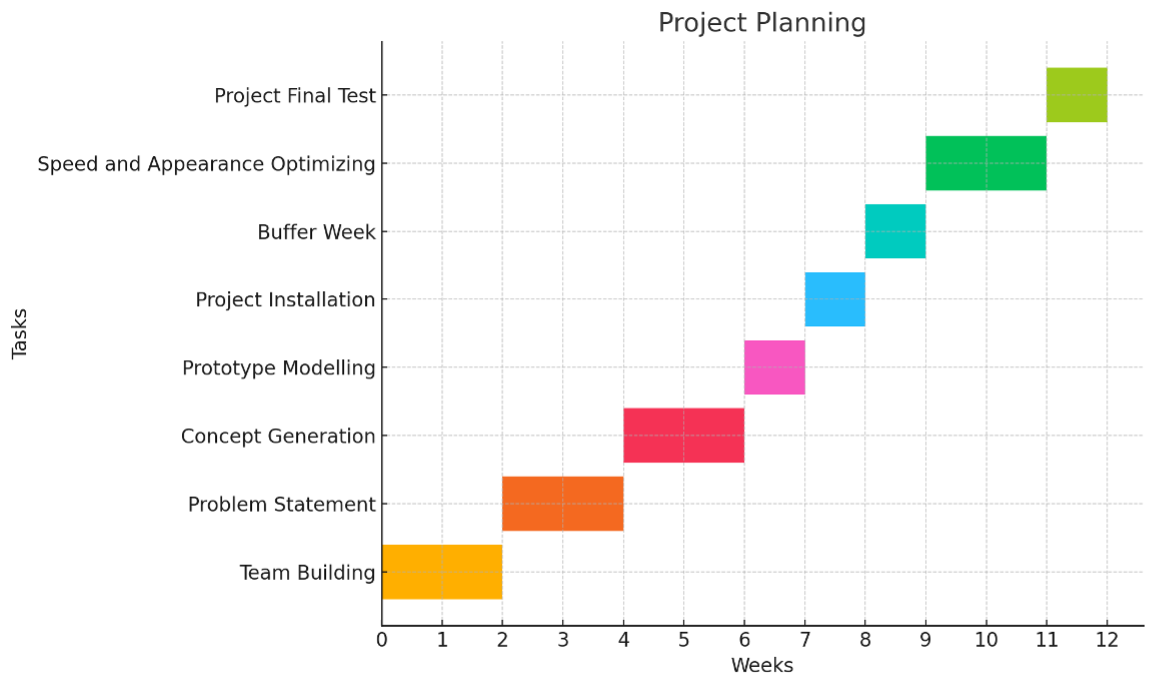
\includegraphics[width=0.8\textwidth]{figure/Picture1.png} % 调整宽度为文本宽度的 50%
    \caption{Gantt Chart} % 添加图片标题
\end{figure}

\begin{table}[h!]
    \centering
    \begin{tabular}{|>{\raggedright\arraybackslash}p{3cm}|>{\raggedright\arraybackslash}p{4.5cm}|>{\raggedright\arraybackslash}p{6cm}|}
        \hline
        \textbf{Responsibility} & \textbf{Assigned Members} & \textbf{Description} \\ 
        \hline
        3D Printing Design Map & Chi-En Peng, Yung-Ching Liang & 
        Accelerates project development and helps achieve precise design outcomes. \\ 
        \hline
        Gearbox & Yaran Zhang, Shenglin Wang & 
        Contains gears, bearings, input shaft, output shaft, and housing. Provides torque amplification and load distribution. \\ 
        \hline
        Power System & Weijia Xiao & 
        Ensures continuous power supply from solar panels to power the car efficiently. \\ 
        \hline
        Organizing  \& Laser Cutting  & Cheong Zhang & 
        Organize the team and assign tasks \&Ensures accurate splicing of frames and reduces material waste. \\ 
        \hline
        Measurement & Yaran Zhang, Yixuan Wu, Chengrui Jiang & 
        Ensures components fit together correctly and machines operate efficiently through precise measurements. \\ 
        \hline
    \end{tabular}
    \caption{Roles and Responsibilities in Solar-Powered Car Project}
\end{table}
\subsection{Previous Work}

In the first six weeks, we completed three theoretical parts: Team Building, Problem Statement, and Concept Generation. In Week 1, team members got to know each other and held the first group meeting, where everyone presented their understanding of the problem statement. In Week 3, the problem statement facilitated more productive group discussions, as the outcomes were more comprehensive and feasible than individual solutions. By Week 5, the team delivered a presentation on concept generation, exploring various materials, power sources, and transmission methods to optimize performance by balancing efficiency, cost, and weight.
\subsection{prototype modeling}
Using a well-equipped car for simple tests was impractical, so we started with temporary substitutes. The body and bottom plate were made of cardboard, with a motor, solar panels, and wheels installed. While the car ran successfully, its speed was unsatisfactory. Additional materials were acquired, and further testing led to design optimizations to reduce weight and improve speed.
\begin{figure}[h] % figure 环境可以让你调整图片的摆放位置
    \centering % 图片居中
    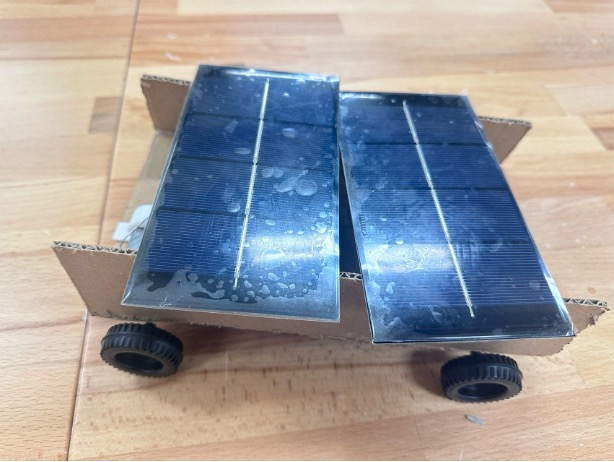
\includegraphics[width=1\textwidth]{figure/car_prototype.jpg} % 调整宽度为文本宽度的 50%
    \caption{Tested Car prototype} % 添加图片标题
\end{figure}
\subsection{Project installation}
To install the car, we have decided the components that may be used in our solar panel car.
Such as the solar panel, DC Motor, wheels, base, the shell, gears, transmission shaft and some wires to transfer electric energy. 
Careful selection and placement of components, such as the solar panel, motor, wheels, and transmission system, is important to ensure a balanced and smooth-running car\cite{Hapuwatte2017}. 
\subsection{Speed and Appearance optimization}
To achieve high speed, we focused on reducing weight and minimizing components. After building the first version, we removed or replaced parts to make it lighter and faster. 
Friction within the power system, including the gearbox and transmission shaft, was minimized. 
On cloudy days, capacitors will power the car, requiring resistor optimization. 
We will also test and adjust the gear ratio to maximize speed. Additionally, the car's appearance will be refined to enhance market appeal.

\subsection{Project Final Test}
In the final test, we aim to have a high speed within competitors. Under the full support of previous test and optimization, we believe our car will have a high speed.
\subsection{Risk Management}
The main risk are shortage of makerspace resource(equipment and material) and installation detail, which could delay the project.
Both risks are mainly affect to the "Project installation" part. To mitigate this risk, we will have a buffer week between the "Project installation" and "Speed and Appearance optimization". 
This week will be used to address the problems and unexpected detail that may occur in the "Project installation" part. 
\subsection{Budget}
\begin{table}[h!]
    \centering
    \begin{tabular}{|>{\raggedright\arraybackslash}p{6cm}|>{\centering\arraybackslash}p{2cm}|>{\centering\arraybackslash}p{3cm}|>{\centering\arraybackslash}p{3cm}|}
        \hline
        \textbf{Item} & \textbf{Quantity} & \textbf{Unit Price (\$)} & \textbf{Total Price (\$)} \\ 
        \hline
        Wheels (40mm) & 4 & 1.40 & 1.40 \\ 
        \hline
        Motor F 18 & 1 & 2.20 & 2.20 \\ 
        \hline
        Toggle switch (two-way, blue) & 1 & 3.00 & 3.00 \\ 
        \hline
        Pinion Gear (10 Tooth) & 1 & 0.30 & 0.30 \\ 
        \hline
        Pinion Gear (12 Tooth) & 1 & 0.30 & 0.30 \\ 
        \hline
        Super Gear (36 Tooth) & 3 & 1.65 & 1.65 \\ 
        \hline
        Super Gear (48 Tooth) & 2 & 1.10 & 1.10 \\ 
        \hline
        Super Gear (54 Tooth) & 2 & 1.10 & 1.10 \\ 
        \hline
        Super Gear (60 Tooth) & 1 & 0.55 & 0.55 \\ 
        \hline
        Spur Gear (48/12 Tooth) & 1 & 0.60 & 0.60 \\ 
        \hline
        Motor Mount (3D printed – Basic) & 1 & 1.00 & 1.00 \\ 
        \hline
        Solar Panel (2V) & 1 & 8.50 & 8.50 \\ 
        \hline
        Ply Wood (for Laser cutter) & 1 & 5.00 & 5.00 \\ 
        \hline
        Capacitor & 1 & 3.65 & 3.65 \\ 
        \hline
        Axle Collar/Bush & 1 & 0.14 & 0.14 \\ 
        \hline
        F/Glass Axle (3mm x 167mm) & 1 & 0.45 & 0.45 \\ 
        \hline
        F/Glass Axle (3mm x 177mm) & 1 & 0.50 & 0.50 \\ 
        \hline
        Other (Double-sided tape, glue, bolts, washers, wire, etc.) & - & 4.00 & 4.00 \\ 
        \hline
        \textbf{Sum} & & & \textbf{35.44} \\ 
        \hline
    \end{tabular}
    \caption{Bill of Materials for Solar-Powered Car}
\end{table}
\section{Summary and Conclusion}

\printbibliography

\end{document}



